\documentclass{article}
\usepackage{vs}

\begin{document}



\lecturetitle{Class 4 - Low Dimensional Vector Search}
\section{Nearest Neighbor Search Definition}

As we have seen, nearest neighbor search is a fundamental computational building block in computer vision, semantic search, data mining, machine learning, and many other applications.

\begin{definition}{\bf Nearest Neighbor Search:} Given a set of points $X = \{x_1,\ldots,x_n\} \in \R^{d}$ 
preprocess them into a data structure of size $\poly(n,d)$ in time $\poly(n,d)$ such that nearest neighbor queries can
be performed. Given a search query point $q$ a radius $r$ and the data structure should return  
return $X_{q,r} = \{i \;\; | \;\; ||q - x_i || \le r \}$. 
\end{definition}
We will later extend this definition in the obvious way to max-inner-product search (MIPS) and cosine similarity search.
Improving the practical and theoretical asymptotic time complexity for computing $X_{q,r}$ is the topic of this class.

*** maybe not necessary to specify poly here since nobody would rpopose an exponential method as the baseline is O(nd) *** 

\begin{center}
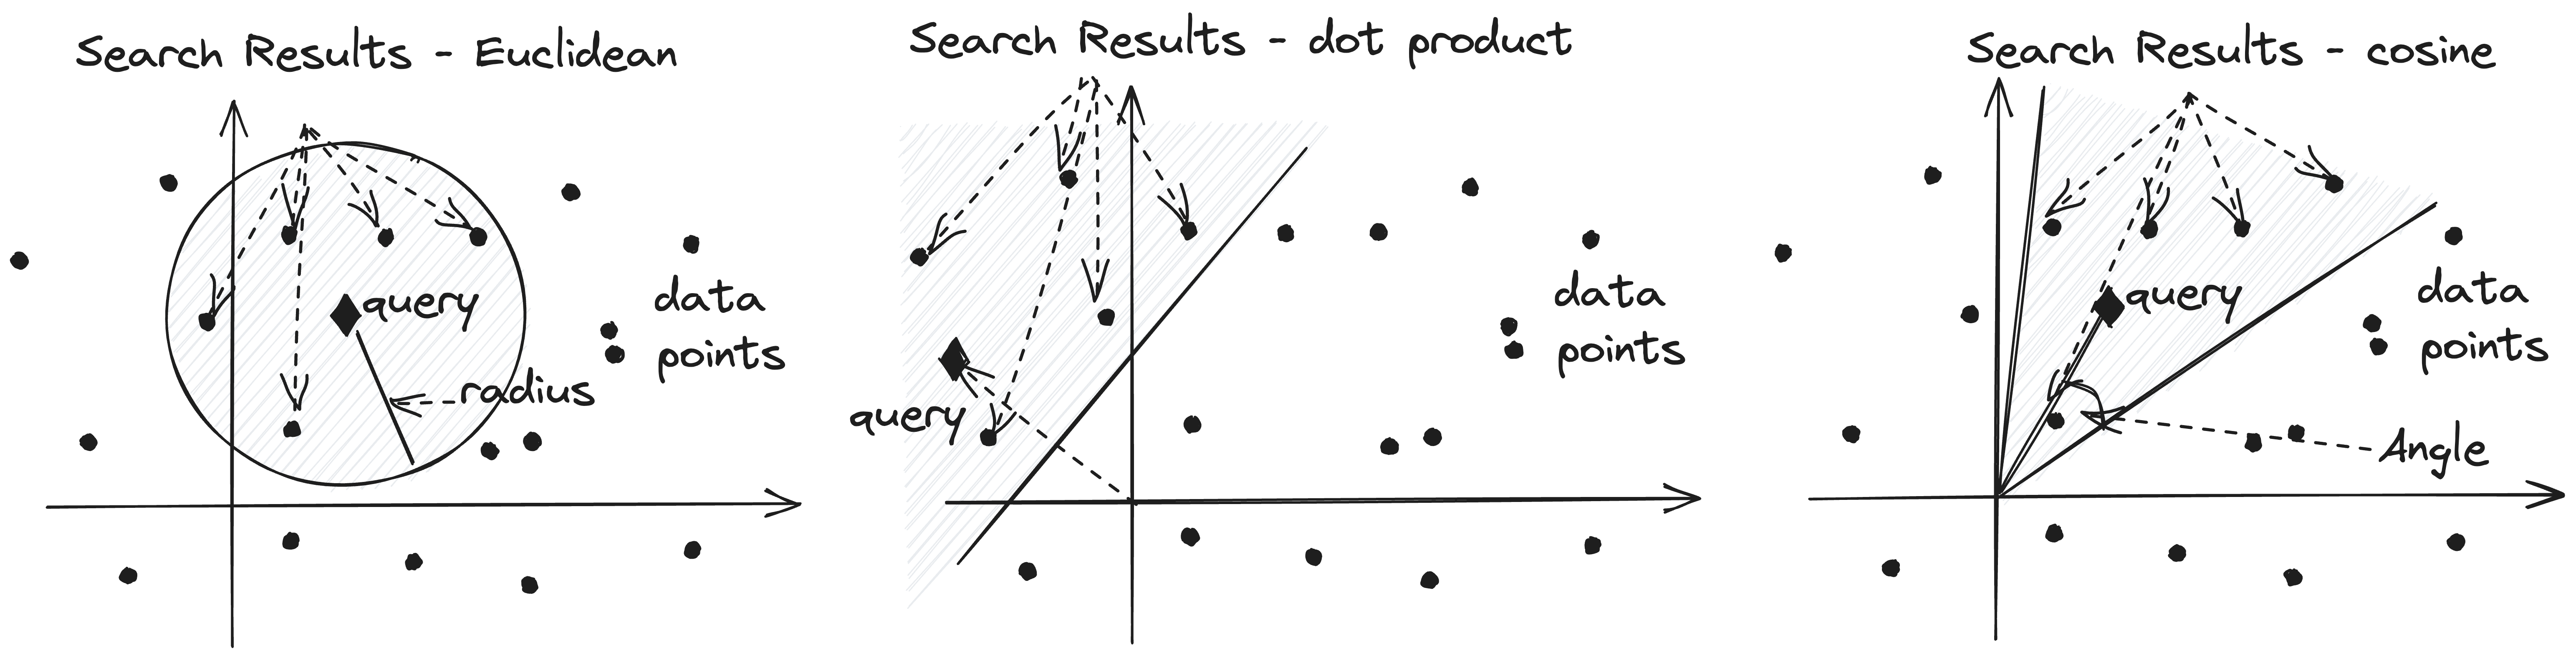
\includegraphics[width=1.0\textwidth]{images/vectorsearch.png}
\end{center}

One option we have is to do nothing at the preprocessing stage. Then, at query time, scan the data points and find those which minimize $\|q - x_i\|$.
This would give a query time of $\Omega(nd)$. But, of course, it would be significantly better if we could reduce the dependence on $n$, or in other words, avoid scanning the data for every query point.

\section{kd-trees}
First, we shall review a well known and widely used algorithm for this problem which is called kd-trees \cite{Bentley75}.
The data structure holds the points in a geometrically partitioned tree. 
Each subtree contains all the points in an axis aligned bounding box,
In each depth in the tree the bounding boxes are split along an axis.
There are many different heuristics for splitting the boxes. For didactic reasons, let's consider a simple construction that lends itself to easy analysis.

In our setting, we assume the number of points is exactly a power of $2$ and that coordinate values are distinct. 
Both assumptions are relatively harmless and should not change the asymptotic behavior. 

We will organize the points in a perfectly balanced binary tree. Points will be associated only with leaves. 
The construction of the tree is simple. We start with all points in a single box (a node in the tree) 
We split the box in two along the first coordinate such that exactly half the points lie on each side. 
The splitting offset is given by the median of these coordinates. 
Then, do the same for each of the two resulting boxes wrt to the second coordinate.
Then, again, for the four resulting boxes wrt to the third coordinate and so on.
Splitting stops when there is exactly one point in each leaf.


\begin{center}
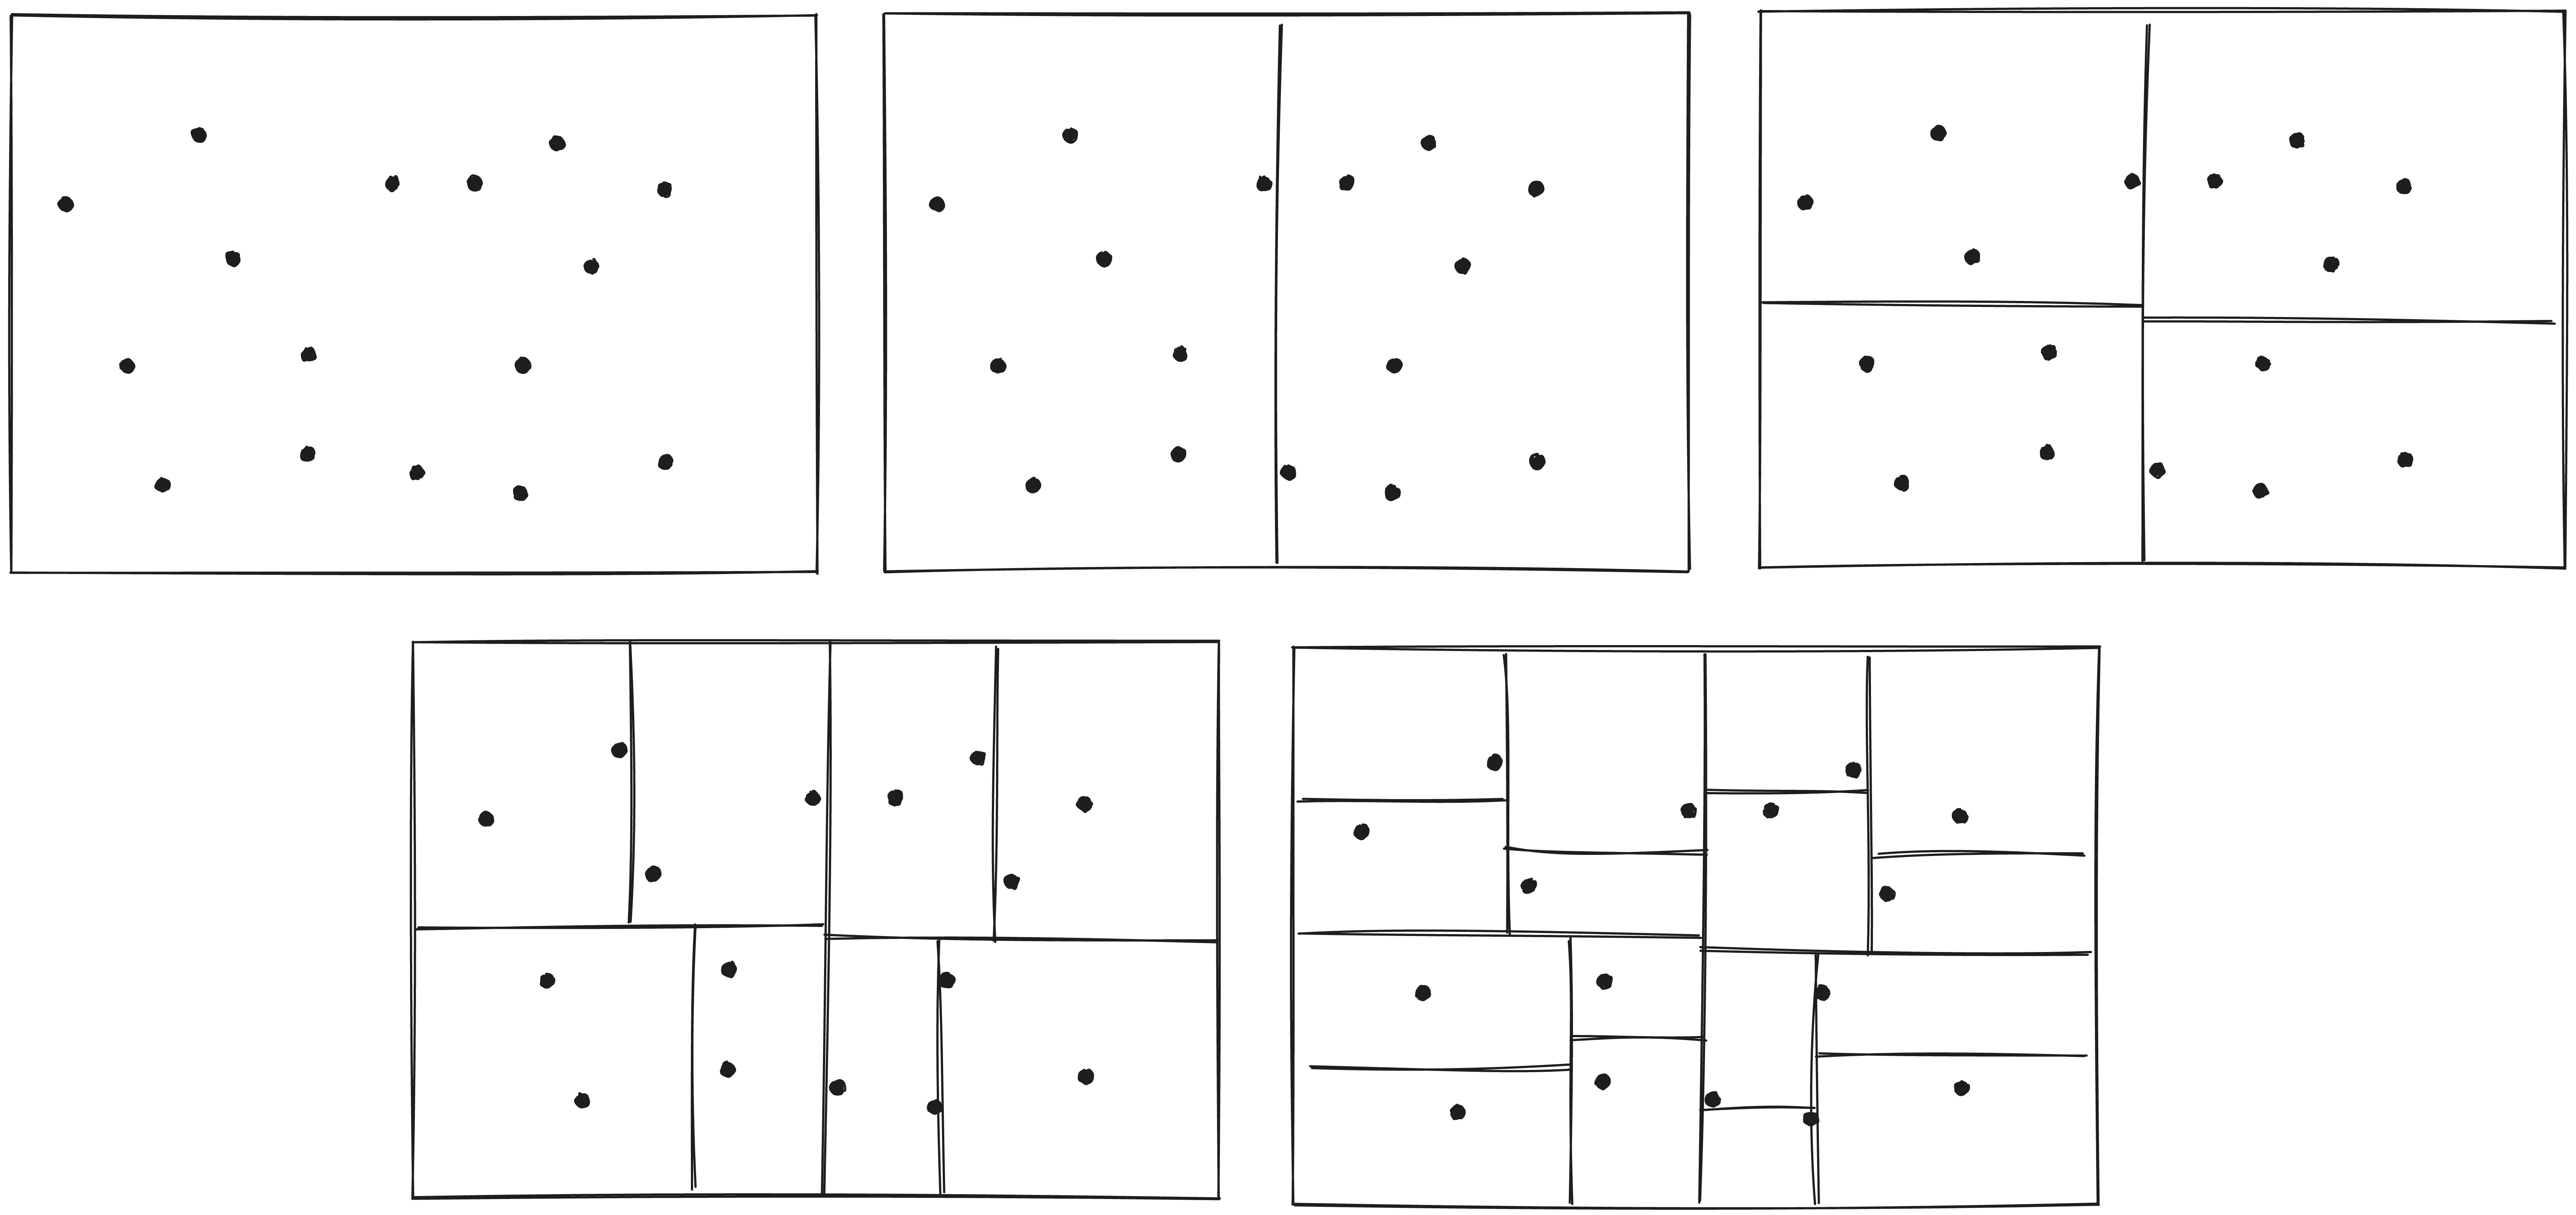
\includegraphics[width=0.9\textwidth]{images/kdtrees-construction.png}
\end{center}


When searching the tree, we consider only points whose bounding boxes touch the query region (ball in this case).

\begin{center}
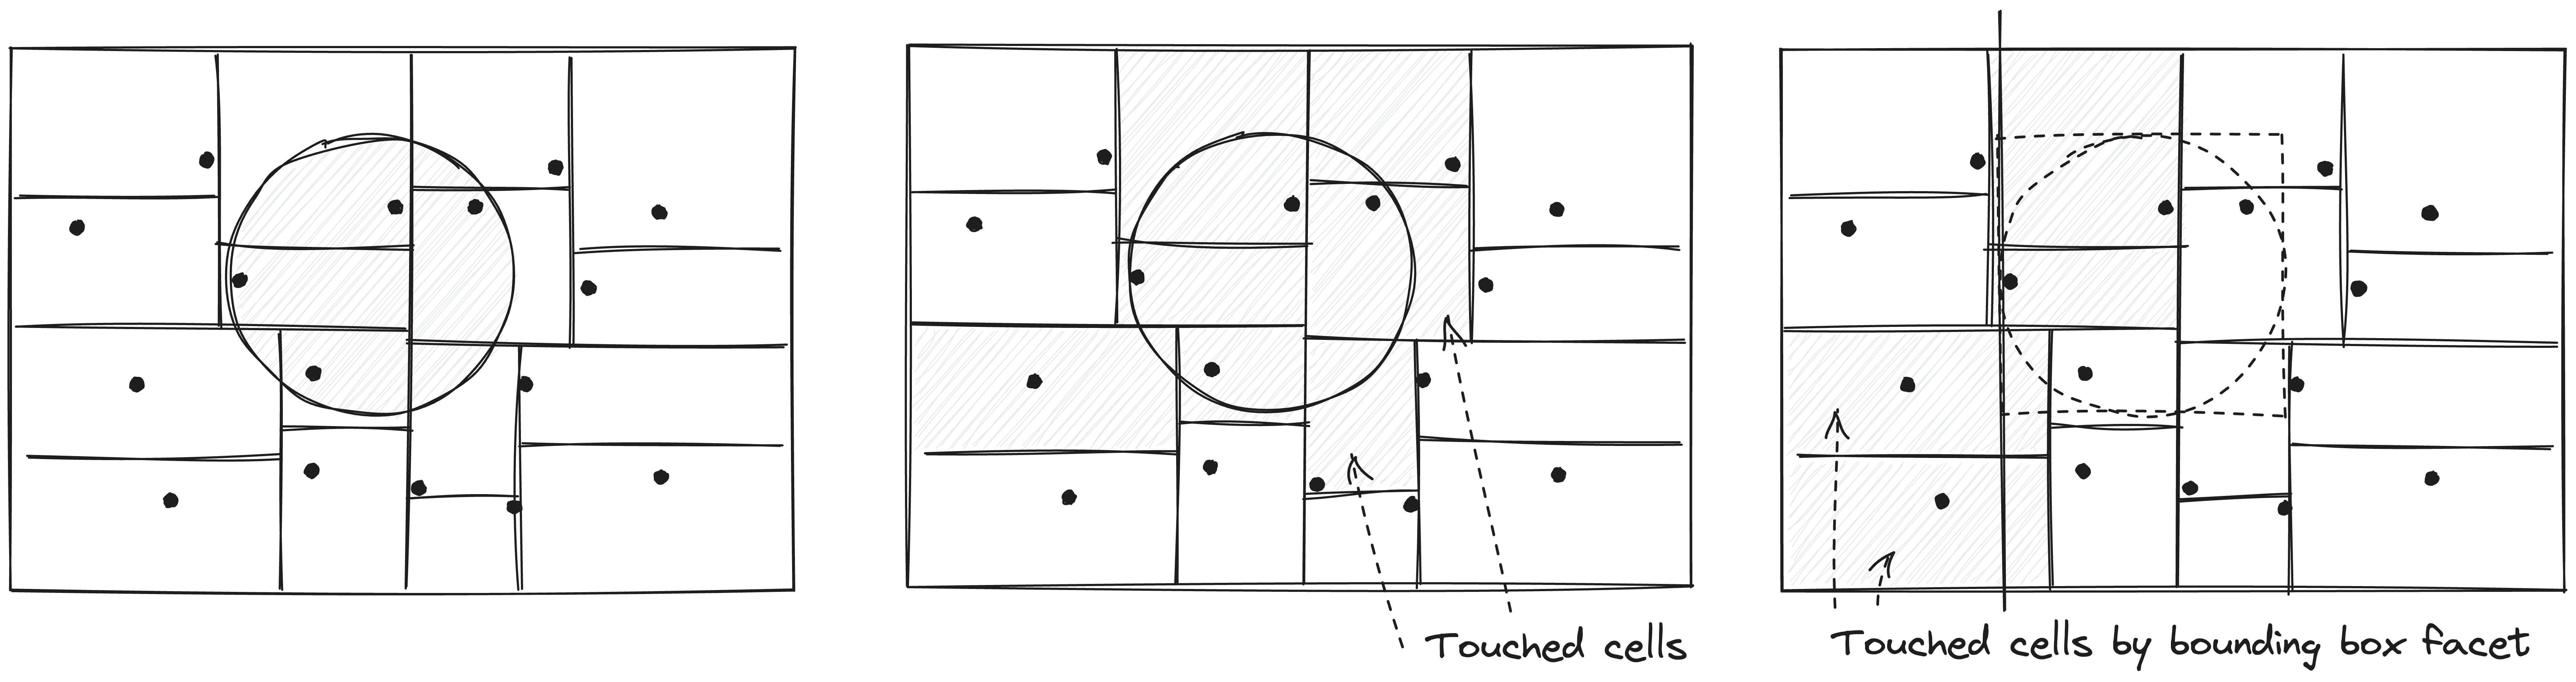
\includegraphics[width=0.9\textwidth]{images/kdtrees-search.png}
\end{center}

\begin{fact}
Any axis aligned hyperplane touches at most $n^{1-1/d}$ boxes.
\end{fact}
\begin{proof}
Assume the hyperplane is aligned with the $i$'th coordinate. That is, the points $x\in\R^d$ such that $x_i = c$. 
When splitting according to coordinate $i$, the split value is either larger or smaller than $c$. 
When that happens, the hyperplane only touches one of the two nodes a level lower in the tree.
The result is that, a splitting according to $i$'s coordinate cuts the number of touched leaf boxes (points) by half.
Finally, since we cycle through the coordinates in a round robin fashion, each coordinate is used for splitting $log_2(n)/d$ times.
Note that $log_2(n)$ is the depth of the tree. We can now calculate the number of touched leaf boxes by $n (1/2)^{log_2(n)/d} = n^{1-1/d}$.
\end{proof}

\begin{center}
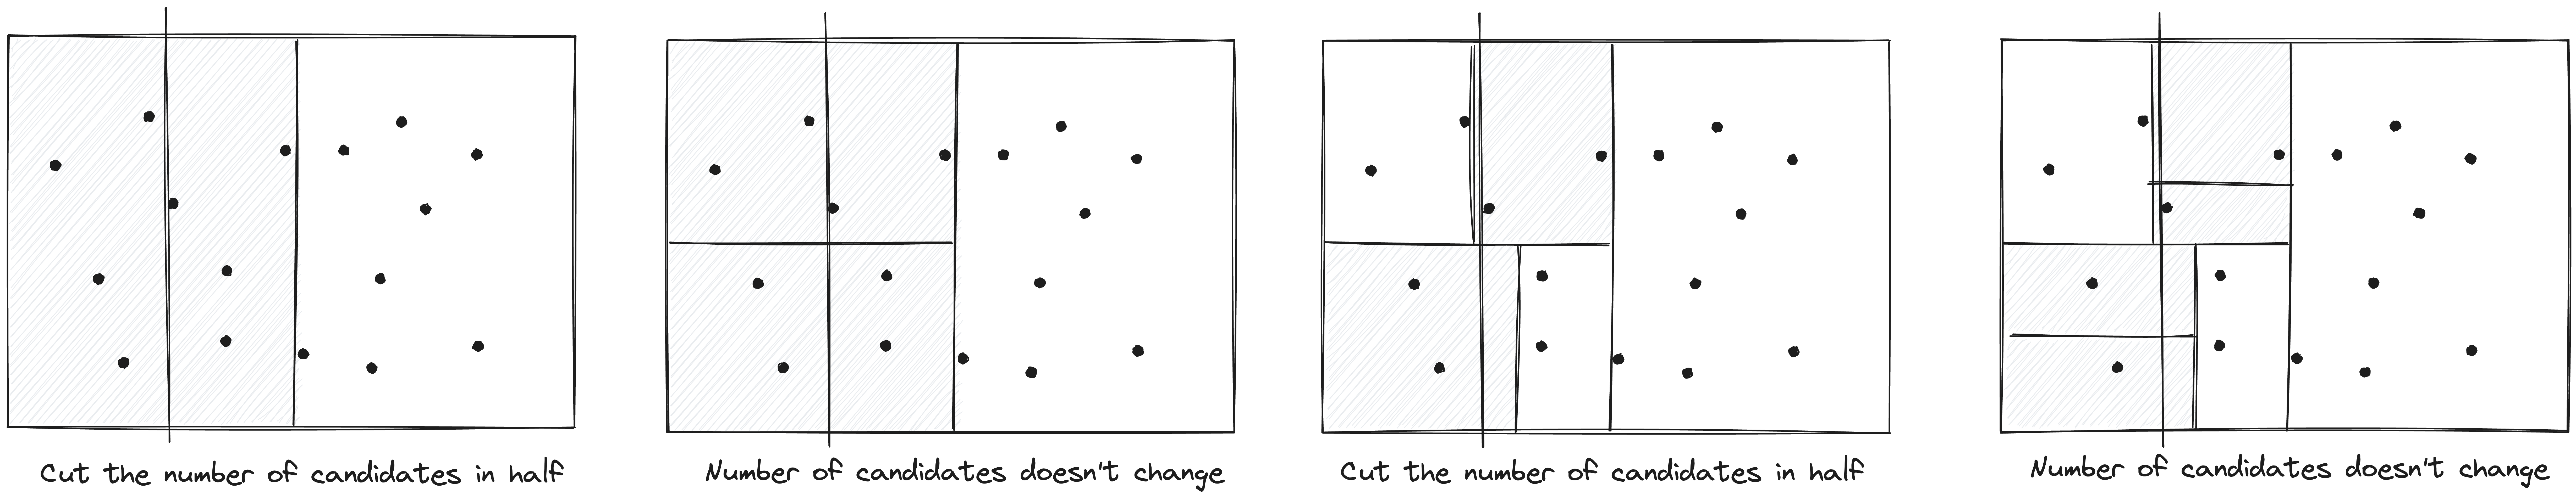
\includegraphics[width=0.9\textwidth]{images/kdtrees-proof.png}
\end{center}

To complete the analysis, note that the axis aligned bounding box of the query has $2d$ facets. Therefore, the number of touched cells is $O(dn^{1-1/d})$.
For each touched cell we need to decide whether the associated point is a valid search result which takes $O(d)$ operations. 
The resulting search complexity of the algorithm is $O(d^2n^{1-1/d})$ which is sub-linear in $n$.
While this analysis is rather simple it actually cannot be made much better  \cite{kdtree-worstcase}. There are many variants of this algorithm \cite{rptrees} and practical observations that claim kd-trees perform well in low dimensions. 

Kd-trees are used extensively in 3D libraries to organize objects, lights, etc. 
They are data adaptive, meaning that they can concentrate on areas where there is data, and keep large boxes when there is not much detail~\cite{subramanian1990search,douze2015quickcsg}. 
In addition to nearest neighbor search they support following rays, organizing data for collision detection, etc. 

\begin{center}
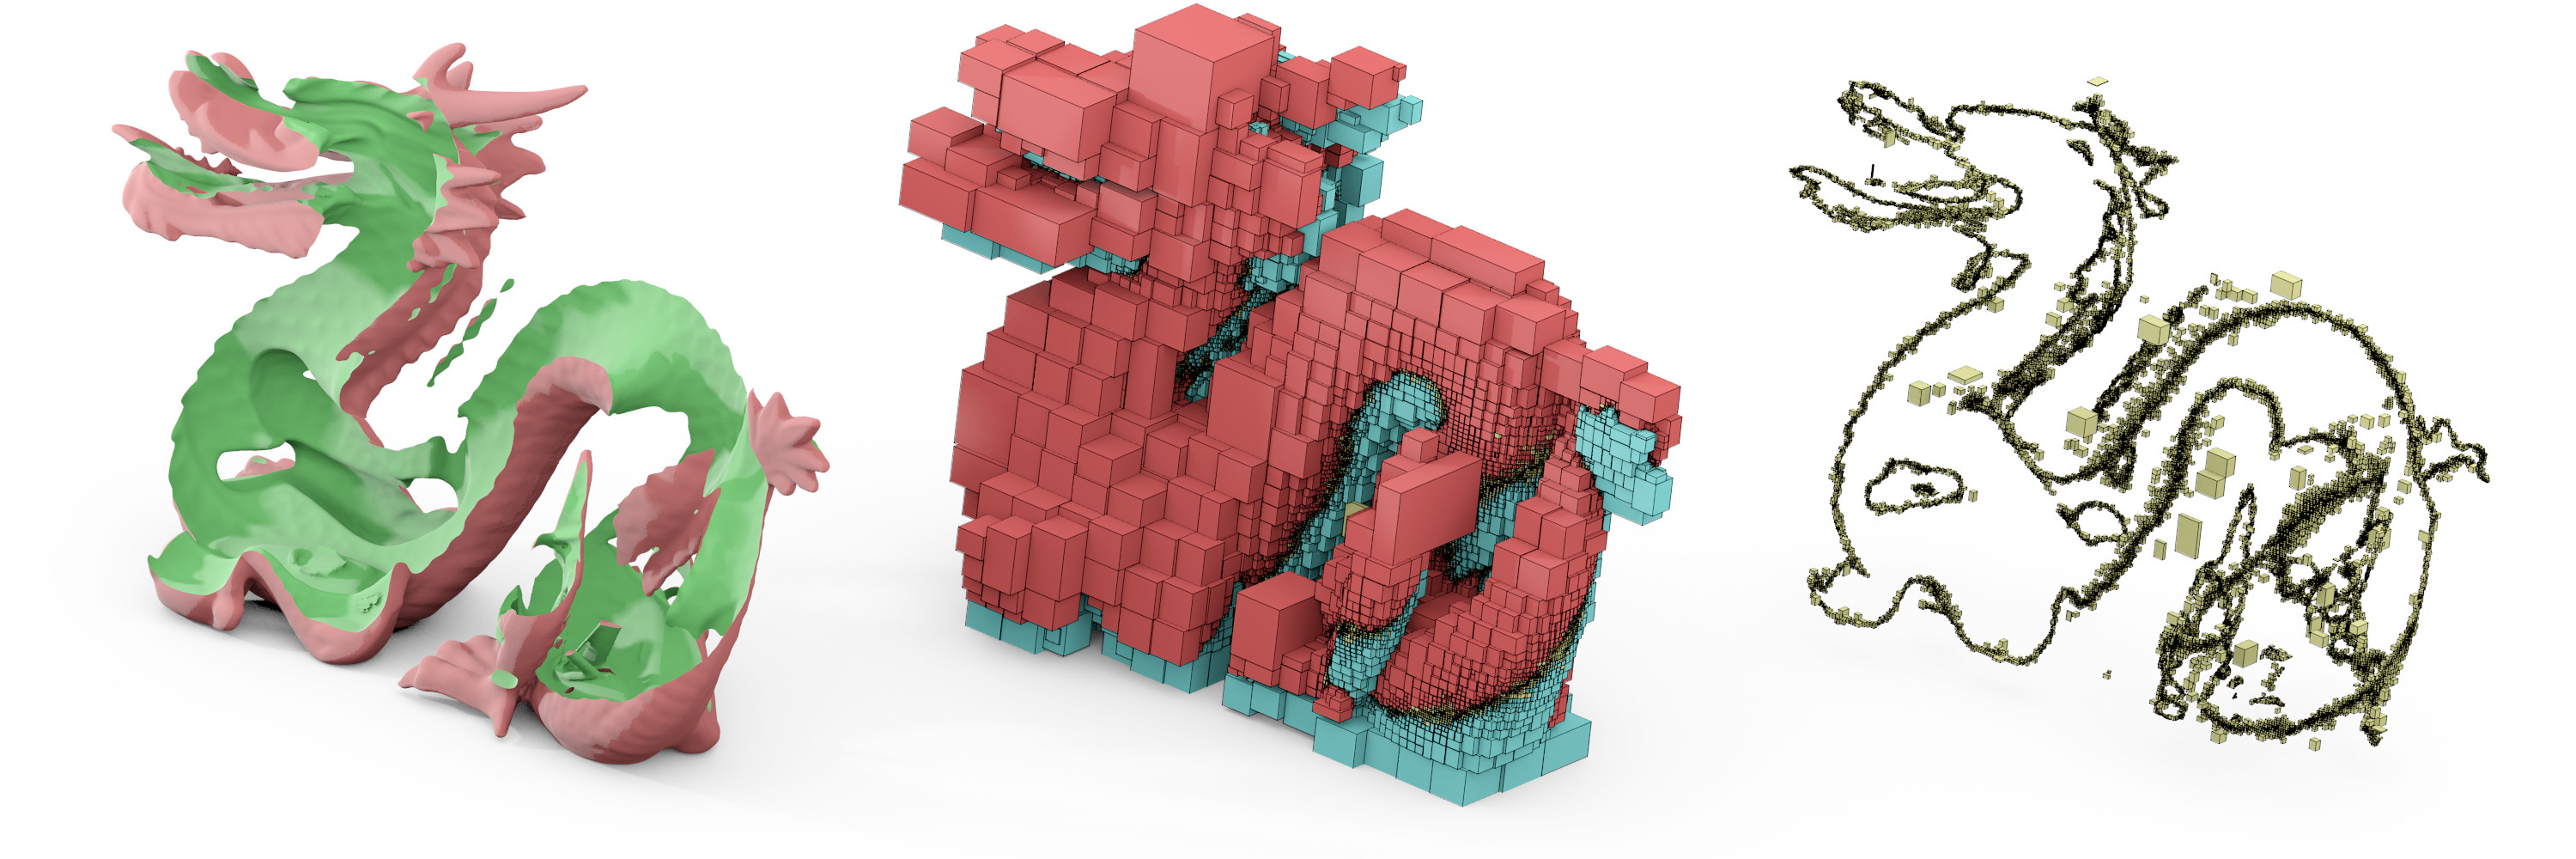
\includegraphics[width=0.9\textwidth]{images/dragon_diff_dup.jpg}
\end{center}


Nevertheless, this runtime is only better than the brute force solution of $O(nd)$ when $n > d^d$ which already hints that there might be a problem with high dimensions.
Before introducing the source of the problem, we should cover some basic facts about random variables. Facts that will serve us for the rest of the course.


\section{Probability Tools and Facts Recap}

A variable $X$ is a random variable if it assumes different values
according to a probability distribution. For example, $X$ can 
denote the outcome of a three sided die throw. 
The variable $X$ takes the values $x = 1,2,3$ with equal probabilities. 

The expectation of $X$ is the sum over the possible values times the probability of the events.
\begin{equation}
\E[X] = \sum_{x=1}^{3}x \Pr(X = x)=
1\frac{1}{3}+2\frac{1}{3}+3\frac{1}{3} = 2
\end{equation}


Continuous scalar random variables are described by their distribution function $\varphi$.
$$
\Pr[Y \in [a,b]] = \int_{a}^{b}\varphi (t) dt.
$$
For a function $\varphi$ to be a valid distribution we must have:
\begin{eqnarray}
\forall \;t, \;\; \varphi(t) &\ge& 0  \mbox{\;\;\; (where it is defined)}\\
\int_{a}^{b}\varphi (t) dt && \mbox{is well defined for all $a$ and $b$}\\
\int_{-\infty}^{-\infty}\varphi (t) dt &=& 1
\end{eqnarray}

For example consider the continuous variable $Y$ taking values in
$[0,1]$ uniformly. That means $\varphi(t) = 1$ if $t \in [0,1]$ and zero else.
This means that the probability of $Y$ being in the interval $[t,t + dt]$ is exactly $dt$. And so the expectation of $Y$ is:
\begin{equation}
\E[Y] = \int_{t=0}^{1}t \varphi(t) dt = \int_{t=0}^{1}t \cdot dt = \frac{1}{2}t^2|_{0}^{1} = 1/2
\end{equation}

\begin{remark}
Strictly speaking, distributions are not necessarily continuous or bounded functions. 
In fact, they can even not be a function at all. 
For example, the distribution of $X$ above includes three Dirac-$\delta$ functions which are not, strictly speaking, functions.
In this class, though, we will see only well behaved distributions.
\end{remark}


\subsection{Dependence and Independence}
A variable $X$ is said to be {\it dependent} on $Y$ if the distribution of $X$ given $Y$ is different than the distribution of $X$. 
For example, assume the variable $X$ takes the value $1$ if $Y$ takes a
value of less than $1/3$ and the values $2$ or $3$ with equal probability otherwise ($1/2$ each).
%
Clearly, the probability of $X$ assuming each of its values is still
$1/3$. However, if we know that $Y$ is $0.7234$ the probability of
$X$ assuming the value $1$ is zero. Let us calculate the expectation of $X$ given $Y$ as an exercise.
\begin{eqnarray}
\E(X | Y) = \sum_{x=1}^{3} x \Pr(X = x | Y \le 1/3) = 1\cdot 1\\
\E(X | Y) = \sum_{x=1}^{3} x \Pr(X = x | Y > 1/3) = 1\cdot 0 + 2
\frac{1}{2} + 3\frac{1}{2}  = 2.5
\end{eqnarray}
$E(X | Y) = 1$ for $y \in [0,1/3]$ and $E(X | Y) = 2.5$ for $y \in (1/3,1]$.\\
Remember: $\E(X | Y)$ is a function of $y$!

\begin{definition}[Independence]
Two variables are said to be {\it Independent} if:
\[
\forall y,\;\;\Pr[ X=x | Y = y] = \Pr[X=x].
\]
They are {\it dependent} otherwise.
\end{definition}


\begin{fact}
If two variables $X$ and $Y$ are {\it Independent} the so are $f(X)$ and $g(Y)$ for any functions $f$ and $g$.
\end{fact}


\begin{fact}[Linearity of expectation 1]%
For any random variable and any constant $\alpha$:
\begin{equation}
\E[\alpha X] = \alpha \E[X]
\end{equation}
\end{fact}

\begin{fact}[Linearity of expectation 2]%
For any two random variables
\begin{equation}
\E_{X,Y}[X+Y] = \E[X] + \E[Y]
\end{equation}
even if they are dependent.
\end{fact}


\begin{fact}[Multiplication of random variables]%
For any two {\bf independent} random variables
\begin{equation}
\E_{X,Y}[XY] = \E[X]\E[Y]
\end{equation}
This does not necessarily hold if they are dependent.
\end{fact}

\begin{definition}[Variance]%
For a random variable $X$ we have 
\begin{equation}
\Var[X] = \E[(X - \E[X])^2] = \E[X^2] - (\E[X])^2
\end{equation}
The standard deviation $\sigma$ of $X$ is defined to be $\sigma(X) \equiv \sqrt{\Var[X]}$.
\end{definition}

\begin{definition}[Additivity of variances]%
For any two {\bf independent} variables $X$ and $Y$ we have 
\begin{equation}
\Var[X + Y] = \Var[X] + \Var[Y]
\end{equation}
\end{definition}

\begin{fact}[Markov's inequality]%
For any {\it non-negative} random variable $X$:
\begin{equation}
\Pr(X > t) \le \frac{E[X]}{t}
\end{equation}
\end{fact}
\begin{proof}
\[
\E_\psi[x] = \int_0^{\infty} z\psi(z)dz = \int_0^{t} z\psi(z)dz + \int_t^{\infty} z\psi(z)dz \ge 0 + \int_t^{\infty} t\psi(z)dz = t \Pr[x>t]
\]
\end{proof}

\begin{fact}[Chebyshev's inequality]%
For any random variable $X$
\begin{equation}
\Pr[|X-E[X]| > t] \le \frac{\sigma^2(X)}{t^2}
\end{equation}
\end{fact}
\begin{proof}
\[
\Pr[|X-E[X]| > t]  = \Pr[(X-E[X])^2 > t^2] \le \frac{\E[(X-E[X])^2]}{t^2} = \frac{\sigma^2(X)}{t^2}
\]
\end{proof}

\begin{lemma}[The union bound]
For any set of $m$ events $A_1,\ldots,A_m$:
\[
\Pr[\cup_{i=1}^{m}A_i] \le \sum_{i=1}^{m}\Pr{A_i}.
\]
\end{lemma}
In words, the probability that one or more events happen is at most the sum of the 
individual event probabilities. 


\begin{theorem}[Chernoff's bound]
Let $X_i$ be a set of {\bf independent} random variables such that $\E[X_i] = 0$ and $|X_i| \le 1$ almost surely.
Also define $\sigma_i^2 = \E[X_i^2]$ and $\sigma^2 = \sum_i \sigma_i^2$. Then:
\[
\Pr[ \sum_i X_i \ge t ] \le max(e^{-t^2/4\sigma^2} , e^{-t/2})
\]
\end{theorem}
\begin{proof}
\begin{eqnarray}
\Pr[ \sum_i X_i \ge t ] &=& \Pr[ \lambda \sum_i X_i \ge \lambda  t ]  \mbox{\;\; (for $\lambda \ge 0$)} \\
&= &\Pr[ e^{\lambda \sum_i X_i} \ge e^{\lambda  t} ]   \mbox{\;\; (because $e^x$ is monotone)} \\
&\le &\E[e^{\lambda \sum_i X_i}] /e^{\lambda  t} \mbox{\;\; (by Markov)} \\
&=& \Pi_i \E[e^{\lambda X_i}] /e^{\lambda  t} \mbox{\;\; (by independence of $X_i$)} 
\end{eqnarray}

\begin{center}
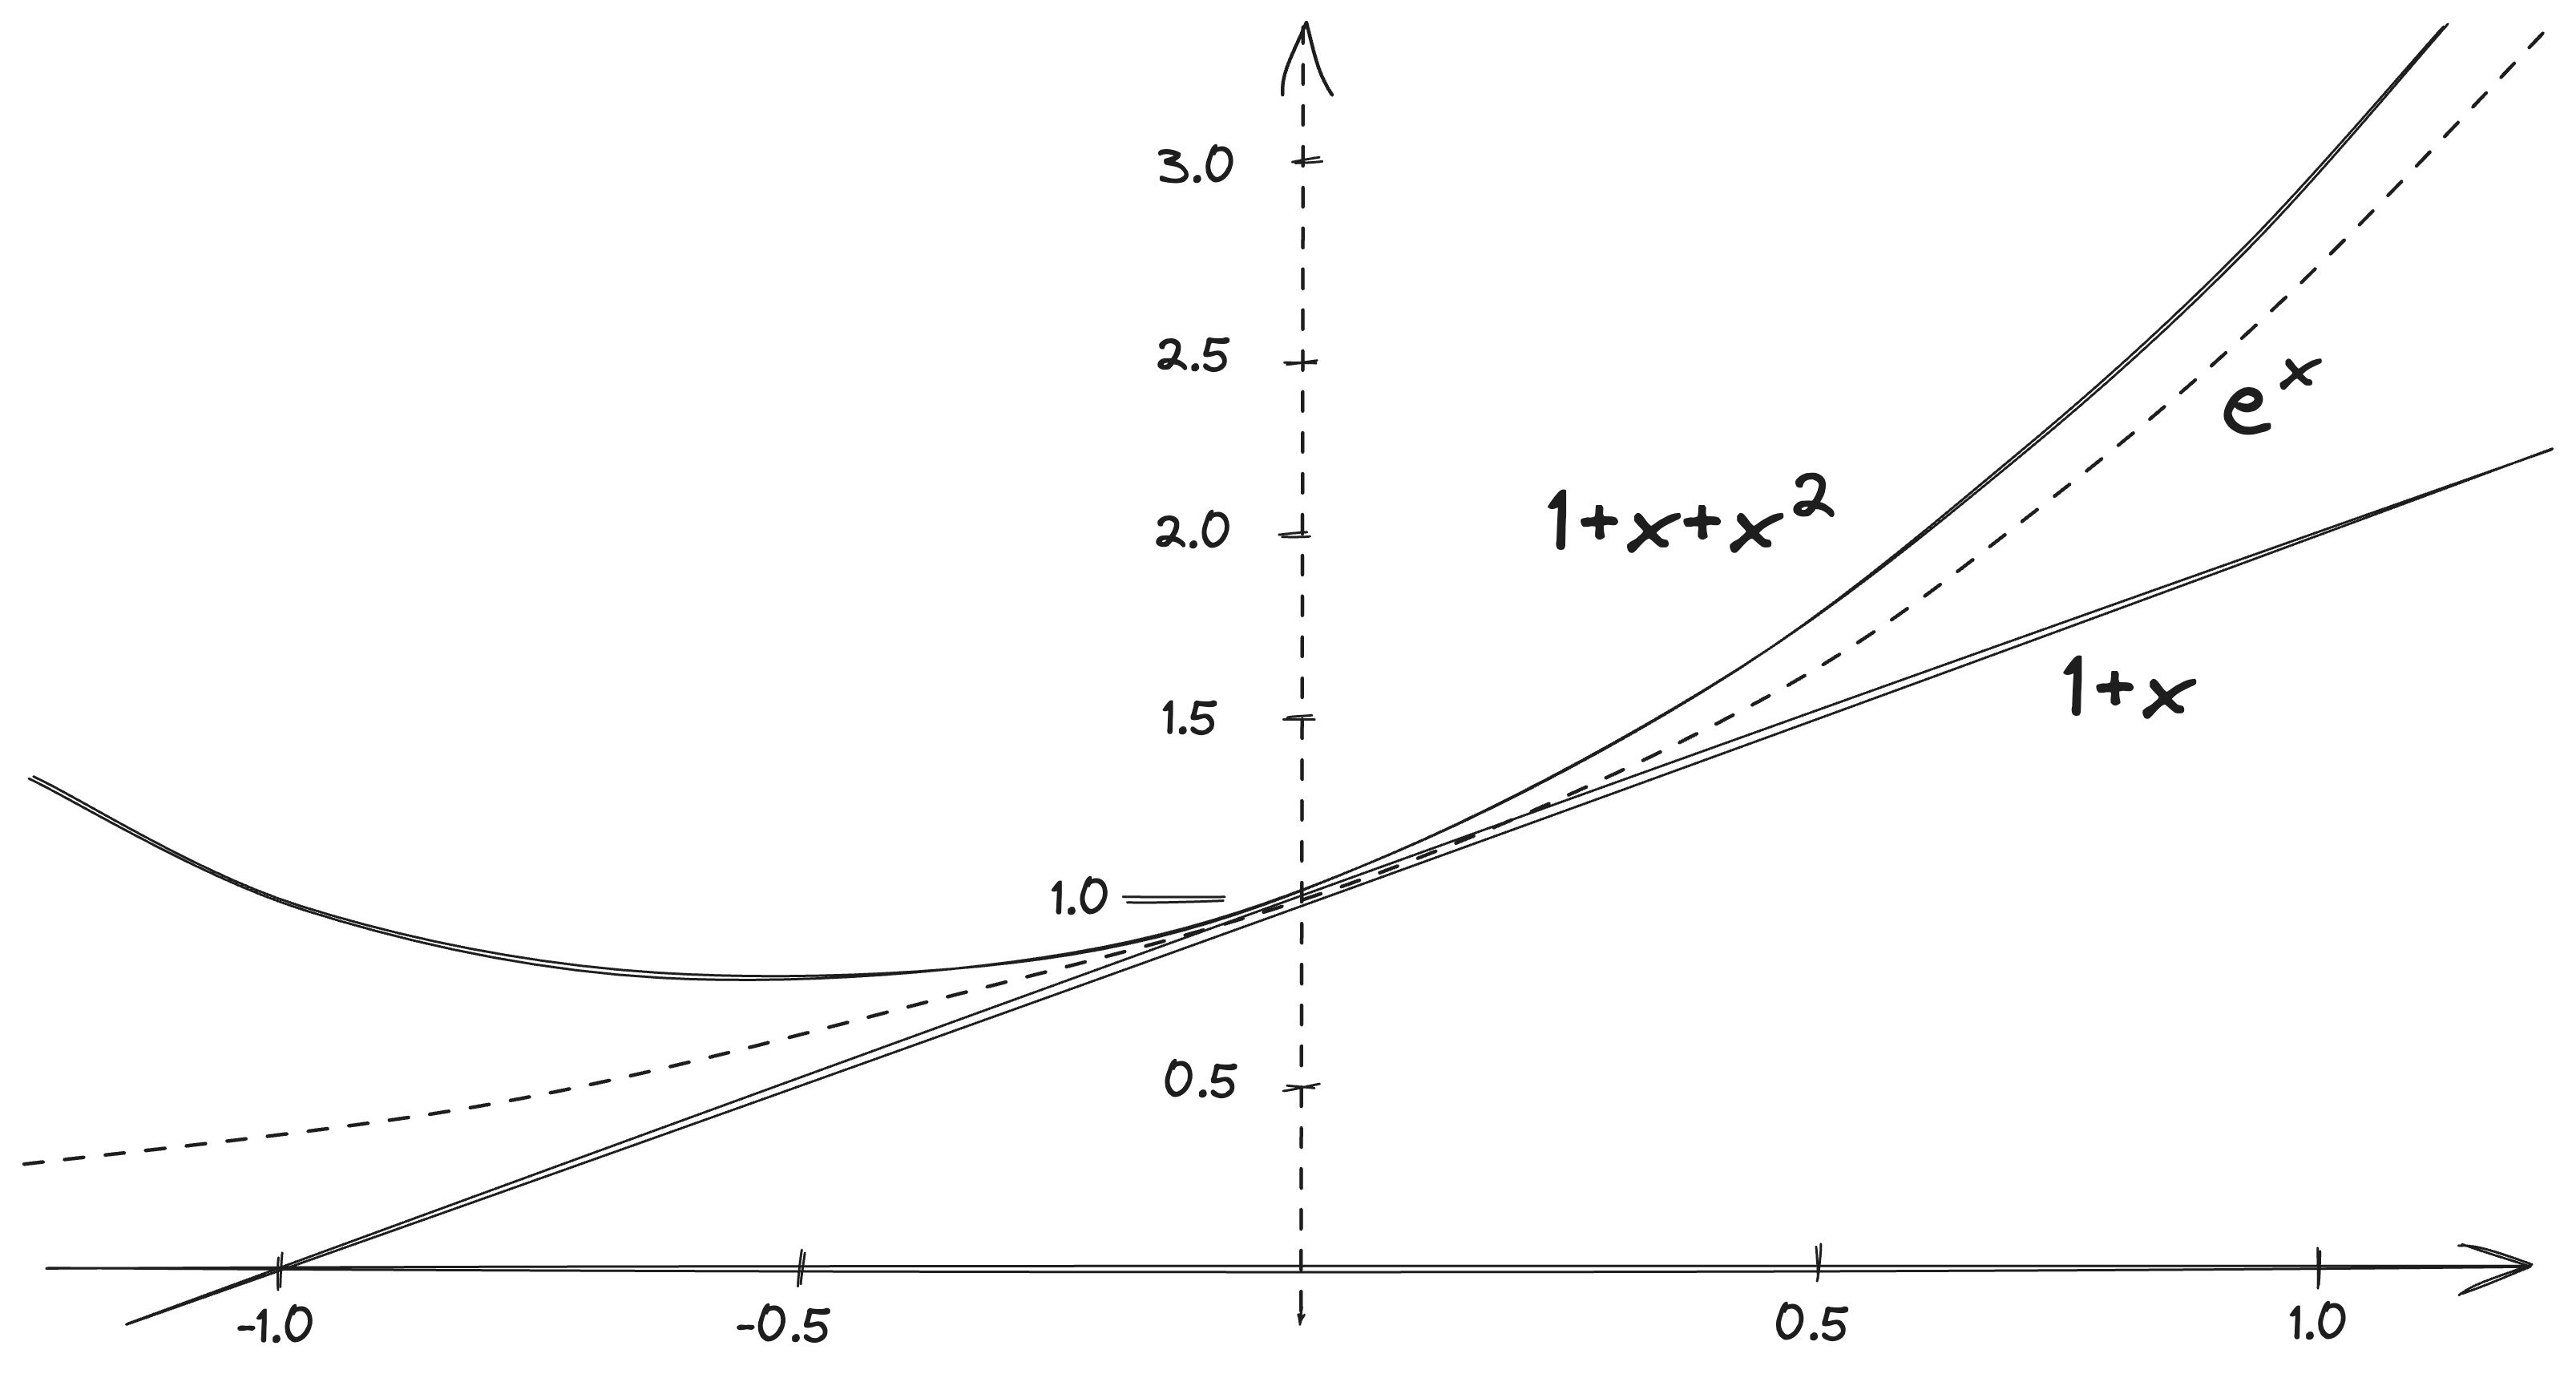
\includegraphics[width=0.5\textwidth]{images/chernoff-exp-bounds.png}
\end{center}

Now, for $x \in [-1,1]$ we have that $e^x \le 1 + x + x^2$ so $\E[e^{\lambda X_i}] \le 1 + \E[\lambda X_i] + \lambda^2 \E[X_i^2] \le 1 + \lambda^2 \sigma^2_i$.
Now, since $1+x \le e^x$ we have that $1 + \lambda^2 \sigma^2_i \le e^{\lambda^2 \sigma_i^2}$. Combining the above we have that $\E[e^{\lambda X_i}] \le e^{\lambda^2 \sigma_i^2}$




\begin{eqnarray}
\Pi_i \E[e^{\lambda X_i}] /e^{\lambda  t} &\le& \Pi_i \E[e^{\lambda^2 \sigma_i^2}] /e^{\lambda  t}\\
&= & e^{\lambda^2 \sigma^2 - \lambda t}
\end{eqnarray}
Now, optimizing over $\lambda \in [0,1]$ we get that $\lambda = min(1,t/2\sigma^2)$ which completes the proof.
\end{proof}

\begin{theorem}[Chernoff's bound; Another useful form]
Let $X_1,\ldots,X_n$ be independent
$\{0,1\}$ valued random variables. Each $X_i$ takes the value $1$
with probability $p_i$ and $0$ else. Let $X = \sum_{i=1}^{n}X_i$ and
let $\mu = E[X] = \sum_{i=1}^{n}p_i$. Then:
\begin{eqnarray*}
\Pr[X > (1+\eps)\mu] &\le& e^{-\mu \eps^2/4}\\
\Pr[X < (1-\eps)\mu] &\le& e^{-\mu \eps^2/2}
\end{eqnarray*}
Or, using the union bound:
\[
\Pr[|X - \mu| > \eps\mu] \le 2e^{-\mu \eps^2/4}
\]
\end{theorem}




\section{Curse of Dimensionality}
A prime example for the curse of dimensionality is that a random point in $[0,1]^d$ is likely to be far from any set of $n$ points in the unit cube.
Consider the distance between the query point $q$ and an input data vector $x$.
We want to show that $\|x_i-q\|^2 \in \Omega(d)$. *** $\Omega(d)$ not defined *** 

First, notice that $\Pr[|x(j)- q(j)| \ge 1/4] \ge 1/2$. The expected distance between $x$ and $q$ is at least $d/8$.
Since $q(j)$ are independently drown, we can apply the Chernoff bound and get that for all $n$ points in the data set
$\|x_i-q\|^2 \ge d/16$ if $d \ge \const\cdot\log(n)$.

Now, consider the kd-tree data structure and algorithm run on a random query.
If the radius of the ball around $q$ is less than $d/16$ the query is ``uninteresting'' since it is likely to return no results at all.
On the other hand, if the radius is greater than $d/16$ than the ball around $q$ will cross all the major partitions 
along one of the axes. That means that the algorithm will visit at least $2^d$ partitions.


\section{Volumes of balls and cubes}
Another interesting phenomenon that occurs in high dimensions is the fact that unit spheres 
are exponentially smaller (in volume) than their containing boxes.
Let us see this without using the explicit formulas for the volume of $d$ dimensional spheres.

To compute the volume of a unit sphere, we perform a thought experiment.
First, bound the sphere in a box (with sides of length $2$).
Then, pick a point in the box uniformly at random. What is the probability $p$ that
the point is also in the sphere? This is exactly the ratio between the volume of the ball and the box ($2^d$).
More accurately, $V = p2^d$ where $V$ is the volume of the sphere.

Now, we can bound $p$ from above. 
A uniformly random chosen point from the cube is a vector $x \in \R^d$ such that each coordinate $x(i)$
is chosen uniformly from $[-1,1]$. The event that $x$ is in the unit sphere is the event that $\|x\|^2 = \sum_{i=1}^{d}x(i)^2 \le 1$.
Let $z_i = x(i)^2$, and note that 
$\E[z(i)] = \int_{-1}^{1}\frac{1}{2}t^2 dt = 1/3$. Therefore, $\E[\|x\|^2] = d/3$. 
Also, 
\[
\var(z_i)  = \int_{-1}^{1}\frac{1}{2}t^4 dt  - (1/3)^2  = 1/5 - 1/9 \le 1/10
\]
so by Chernoff's inequality.
$p = \Pr[\sum_{i=1}^{d}x(i)^2 \le 1]  = \Pr[\sum_{i=1}^{d}(z_i -\E[z_i] ) \le 1-d/3] \le e^{-\frac{(d/3)^2}{4d/10}} \le e^{-d/4}$.
This concludes the observation that the fraction of the volume which is inside the sphere is 
exponentially small compared to the cube.
A counter intuitive way of viewing this is that almost the entire volume of the cube is concentrated at the ``corners".

\section{Orthogonality of random vectors}

It turns out that two random vectors are also almost orthogonal.
We can see this in two ways.

First, we can see that the expected dot product of any vector $x$ with a random vector $y$ is small.
It is trivial that $\E[\langle x,y \rangle] = 0$ since the distribution of $y$ is symmetric.
*** what is the condition on the data distribution? We sometimes have positive vectors \. Seems that this is random vectors on unit sphere or Gaussian isotropic *** 
Moreover, $\E[\langle x,y \rangle^2] = 1/d$.
To see this, consider $y_1,y_2,\ldots,y_d$ where $y_1 = y$ and $y_2,\ldots,y_d$ complete $y$ to an orthogonal basis.
Clearly, the distribution of all $y_i$ are identical (but not independent)
$\E[\langle x,y \rangle^2] = \E[\langle x,y_1\rangle^2] = \E[\frac{1}{d}\sum_{i=1}^{d}\langle x,y_i\rangle^2] = \frac{1}{d}\|x\|^2 = \frac{1}{d}$.

It is not hard to show that in fact for any vector $x$, if $y$ is chosen uniformly at random from the unit sphere 
then $\Pr[ \langle x,y \rangle  \ge \frac{t}{\sqrt{d}}] \le e^{-t^2/2}$.
First, replace that uniform distribution over the unit sphere with an i.i.d. distribution of Gaussians $y(i)\sim \N(0,\frac{1}{\sqrt{d}})$.
Note that $E[\|y\|^2] = 1$, moreover, from the sharp concentration of the $\chi^2$ distribution we know that $E[\|y\|^2] \approx 1$.
For convenience we will assume that $E[\|y\|^2] = 1$ and will ignore the small inaccuracy.
Moreover, due to the rotational invariance of the Gaussian distribution we have that any direction is equally likely and thus this
new distribution approximates the uniform distribution over the sphere.
Next, notice that due to the rotational invariance $\langle x,y \rangle \sim \N(0,\frac{\|x\|}{\sqrt{d}}) = \N(0,\frac{1}{\sqrt{d}})$.
Therefore, letting $Z \sim \N(0,1)$ we have $\Pr[ \langle x,y \rangle  \ge \frac{t}{\sqrt{d}}] = \Pr[Z \ge t] \le e^{-t^2/2}$.


\section{The failure of space partitioning schemes}
As we've seen, a ``typical'' distance from a random query to the nearest neighbor in a $d$-dimensional unit box is at the scale of $\sqrt{d}$.
Note that the side of any box in any space partitioning scheme (including kd-trees, of course) is at most $1$. 
As a result, we guaranteed to scan at least $\Omega(d)$ levels in the tree which is $\exp(d)$ points.
Note that this is more than the brute force solution of $O(nd)$ when $d > \log(n)$. 
*** this is a contradiction because the tree depth is also limited by the number of points in the dataset. What is interesting is that beyond some dimension, the tree leaves are "open", ie. not all borders are closed by a hyperplane *** 




\bibliographystyle{plain}
\bibliography{vs}

\end{document}
%%%%%%%%
